\documentclass{article}
\usepackage{graphicx}
\usepackage[utf8]{inputenc}
\usepackage[fleqn]{amsmath}
\usepackage{titling}
\usepackage{graphicx,wrapfig,lipsum}
\usepackage{amssymb}
\usepackage{listings}
\usepackage[font=small,labelsep=none]{caption}
\usepackage{hyperref}
\usepackage{caption}

\setlength{\droptitle}{-10em}
\setlength\parindent{0pt}

\title{Project 3}\vspace{-3ex}
\author{Benedicte Allum Pedersen, Emil Heland Broll\\ Fredrik Oftedal Forr}
\date{\vspace{-5ex}}

\begin{document}
\maketitle

\section*{Abstract}



\section*{Introduction}
In this report there were given a brief rundown on different numerical integration methods. The methods that have been used is Gauss-Legendre and Gauss-Laguerre quadrature as well as Monte Carlo integration. There will be adjustments to these to show the different strengths of the methods. Under this paragraph you can find the method on how the program works, results from the program, discussion where we analyze the results and ending with a conclusion.\\

The integral we have worked with is a six-dimensional integral which determines the ground state correlation energy between two electrons in a helium atom.\\

The single-particle wave function for an electron $i$ in the $1s$ state in a hydrogen atom is as followed:

\begin{flalign*}
  \psi_{1s}(\textbf{r}_i)= e^{- \alpha r_i}
\end{flalign*}

where $\textbf{r}_i = x_i \textbf{e}_x + y_i \textbf{e}_y + z_i \textbf{e}_z +$, and the value of $r_i$ is given by:

\begin{flalign*}
  r_i = \sqrt{x_i^2 + y_i^2 +z_i^2}
\end{flalign*}

We set $\alpha = 2$ which corresponds to the charge of the helium atom, Z = 2. We assume that the wave function for each electron in the helium atom can be modelled like the single-particle wavefunction above. The wavefunction for two electron is then given bye the product of two single-particle wavefunctions:

\begin{flalign*}
  \Psi(\textbf{r}_1, \textbf{r}_2) = e^{-\alpha(r_1 + r_2)}
\end{flalign*}

We need to solve the intergral for the expectation value of the correlation energy between two electrons:

\begin{flalign*}
  \left<\frac{1}{|\textbf{r}_1 - \textbf{r}_2|}\right> = \int_{-\infty}^{\infty} d\textbf{r}_1 d\textbf{r}_2 e^{-\alpha(r_1 + r_2)} \frac{1}{|\textbf{r}_1 - \textbf{r}_2|}
\end{flalign*}

The exact value of this integral is $
5\pi^2/16^2 = 0.192765$.


\section*{Method}
In this problem there have been used c++ as programming language and mainly a variety of functions to solve the integral.

\subsection*{Gaussian Quadrature}
To compute the integral numerically we do the approximation:

\begin{flalign*}
  I = \int_{a}^{b} f(x) dx = \int_{a}^{b} W(x)g(x) dx \approx \sum_{i=1}^{N} \omega_i f(x_i)
\end{flalign*}

Unlike other more basic methods for numerical integrations where the mesh points $x_i$ are equidistantly spaced, the mesh points in the gaussian quadrature are not equidistantly spaced. In the sum above $w_i$ correpsonds to the weights. Gaussian quadrature uses some orthonogonal Legendre- and Laguerre-polynomials, to obtain the mesh points and weights.\\

Gauss-Legendre is a brute-force method and to obtain the value of the integral using this method we have to set up the mesh points and weights that corresponds to some finite integrations limits [a, b]. To set up the mesh points and weights we haved used the function $gauleg$ from Morten's \href{https://github.com/CompPhysics/ComputationalPhysics/blob/master/doc/Projects/2019/Project3/CodeExamples/exampleprogram.cpp}{exampleprogram.cpp}.\\

While the Legendre polynomials are defined for $x \in [-1, 1]$ the Laguarre polynomials are defined for $x \in [0, \infty)$. We rewrite the integral and change to spherical coordinates.

\begin{falign*}
  d\textbf{r}_1d\textbf{r}_2 = r_1^2dr_1r_2^2dr_2dcos(\theta_1)dcos(\theta_2)d\phi_1d\phi_2
\end{falign*}

So the integral becomes:\\

\begin{flalign*}
  I = \int_0^\infty r_1^2dr_1 \int_0^\infty r_2^2dr_2 \int_0^\pi dcos(\theta_1) \int_0^\pi dcos(\theta_2) \int_0^{2\pi} d\phi_1 \int_0^{2\pi} d\phi_2 \frac{e^{-2\alpha(r_1+r_2)}}{r_{12}}
\end{flalign*}

where

\begin{flalign*}
  \frac{1}{r_{12}} = \frac{}{\sqrt{r_1^2 + r_2^2 - 2r_1r_2cos(\beta)}}
\end{flalign*}

with

\begin{flalign*}
  cos(\beta) = cos(\theta_1)cos(\theta_2) + sin(\theta_1)sin(\theta_2)cos(\phi_1 - \phi_2)
\end{flalign*}

We perform the integration over $\theta \in [0, \pi]$, $\phi \in [0, 2\pi]$ and $r \in [0, \infty)$. To calculate the mesh points and weight for the angles we use the same function as for the Gauss-Legendre quadrature. To calculate the mesh points and weights corresponding to $r_1$ and $r_2$ we use Morten's function \href{https://github.com/CompPhysics/ComputationalPhysics/blob/master/doc/Projects/2019/Project3/CodeExamples/gauss-laguerre.cpp}{gauss$\_$laguerre.cpp}.

\subsection*{Monte Carlo integration}
Monte Carlo integration allows us to make a good approximation to

\section*{Results}

We have plotted the wave function for the electrons in the Helium atom in figure \ref{fig:wavefunc}. From this plot we can tell that the integral converges to zero for $-2 > x > 2$. Therefore the integral would not need to be evaluated for those values of x.

\begin{figure}[hbt]
\begin{center}
    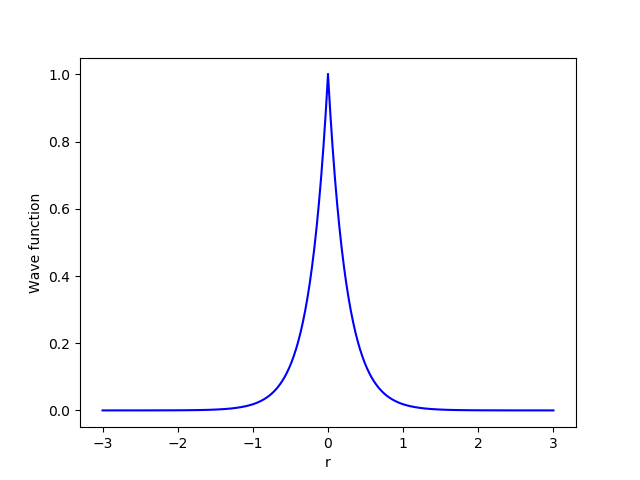
\includegraphics[width=200px]{Wave_func.png}
    \caption{: Plot of the wave function for to electron in a Helium atom.}
    \label{fig:wavefunc}
\end{center}
\end{figure}

Table \ref{Tab: Legendre} and table \ref{Tab: Laguerre} shows the results for the two Gaussian quadratures with different values of N. The tables also shows the difference from the exact value of the integral, namely 0.192765. You can also see a plot of the difference from the exact value for Gauss-Legendre and Gauss-Laguerre in figure

\begin{table}[h!]
  \caption{: Integration using Gauss-Legendre, variying N}
  \begin{tabular}{c c c}
    N & Legendre & Diff. from exact \\
    \hline
    10 & 0.071980 & 0.120785 \\
    15 & 0.239088 & 0.046323 \\
    20 & 0.156139 & 0.036626 \\
    25 & 0.196817 & 0.003052 \\
    27 & 0.193524 & 0.000759 \\
    30 & 0.177283 & 0.015482 \\
  \end{tabular}
  \label{Tab: Legendre}
\end{table}

\begin{table}[h!]
  \caption{: Integration using Gauss-Laguerre, variying N}
  \begin{tabular}{c c c}
    N & Laguerre & Diff. from exact \\
    \hline
    10 & 0.177081 & 0.0156840 \\
    15 & 0.193285 & 0.000520 \\
    20 & 0.194786 & 0.002021 \\
    25 & 0.194804 & 0.002039 \\
    27 & 0.193524 & 0.002030 \\
    30 & 0.194779 & 0.002014 \\
  \end{tabular}
  \label{Tab: Laguerre}
\end{table}



\section*{Discussion}


\section*{Conclution}

\section*{Appendix}


\section*{Bibliography}


\end{document}
